\chapter{Wstęp teoretyczny}
\label{cha:wstepTeoretyczny}

%---------------------------------------------------------------------------

\section{Procesy biznesowe}
\label{sec:procesyBiznesowe}

\subsection{Procesy biznesowe}
W każdym dużym przedsiębiorstwie każdego dnia wykonywana jest ogromna ilość czynności koniecznych do funkcjonowania tej organizacji. Ludzie oraz systemy realizują rozmaite działania związane z różnymi, często niemającymi wiele wspólnego zadaniami jak, chociażby procesowanie płatności, składnie zamówień, wytwarzanie produktów czy ich transport. Przykłady te można mnożyć w zależności od sektora, w jakim obraca się dana firma. Im jest ona większa, tym trudniej jest osobom nią zarządzającym zrozumieć i opisać poszczególne czynności. W pewnym momencie, kiedy ilość różnych zadań rośnie do setek czy tysięcy, staje się to niemożliwe i potrzebny jest sposób na zebranie wiedzy o pojedynczych operacjach i zamknięcie ich w uporządkowaną strukturę. Stąd narodził się pomysł na wykorzystanie procesów biznesowych.

Procesy biznesowe opisują zbiór aktywność, które podejmuje grupa podmiotów w celu osiągnięcia celu biznesowego. W literaturze brakuje jednej ogólnie przyjętej definicji procesu biznesowego. W latach 90. XX wieku proponenci BPR, czyli przeprojektowania procesów biznesowych (\textit{eng. business process re-engineering}) starali się sprecyzować pojęcie procesu biznesowego. W książce ,,Process Innovation: Reengineering Work through Information Technology'' \cite{davenport1993process} określono termin ten jako: ,,Ustrukturyzowany, mierzalny zbiór działań, których celem jest wytworzenie określonego produktu dla określonego klienta lub rynku''. Autor położył nacisk na zbiór kroków prowadzących do celu, raczej niż na końcowy efekt. W dalszej części podsumowano: ,,Proces jest zatem określonym uporządkowaniem czynności roboczych w czasie i przestrzeni, z początkiem i końcem oraz jasno określonymi wejściami i wyjściami: strukturą działania.''. Inni pionierzy BPR Michael Hammer i James Champy zaproponowali  podejście: ,,Proces biznesowy to zbiór działań, który pobiera jeden lub więcej rodzajów danych wejściowych i tworzy wynik, który ma wartość dla klienta'' \cite{HAMMER199390}. Autorzy dają większą dowolność, co do definicji procesu, nie wspominając o konieczności jego logicznej organizacji czy mierzalności. Z kolei Ivar Jacobson zupełnie pomija konieczność zamknięcia procesu w jakiekolwiek ramy, określając go jako: ,,Zestaw czynności wewnętrznych wykonywanych w celu obsługi klienta'' \cite{JacobsonObjectAdvantage}. Nacisk na konieczność odniesienia procesów do wymiernych środków firmy widzimy w definicji: ,,Procesy biznesowe są aktywną częścią biznesu. Opisują funkcje firmy i obejmują zasoby, które są używane, przekształcane lub wytwarzane. Proces biznesowy to abstrakcja, która pokazuje współpracę między zasobami i transformację zasobów w biznesie. Podkreśla, w jaki sposób wykonywana jest praca, zamiast opisywać produkty lub usługi wynikające z tego procesu.'' \cite{Eriksson2000BusinessMW}. Szczególnie ważny jest tutaj fragment o transformacji zasobów, gdyż każe on rozumieć poszczególne aktywności w procesie jako powiązane ze sobą i kończące się namacalnymi rezultatami. Definicja ,,Proces biznesowy to seria kroków mających na celu wytworzenie produktu lub usługi. W wyniku niektórych procesów produkt lub usługa jest odbierana przez zewnętrznego klienta organizacji. Nazywamy je podstawowymi procesami. Inne procesy wytwarzają produkty, które są niewidoczne dla klienta zewnętrznego, ale są niezbędne do efektywnego zarządzania firmą. Nazywamy je procesami wsparcia'' \cite{rummler_brache_1995} wprowadza rozgraniczenie na podtypy procesów. Ważnym jest jednak, że nie jest koniecznością, aby rezultaty procesu były widoczne na zewnątrz organizacji. Warto też zaznaczyć, że procesy biznesowe nie dotyczą jednej osoby czy nawet działu, a raczej udział w nich bierze wiele ludzi, maszyn czy systemów z różnych działów połączonych celem dostarczenia wspólnej wartości biznesowej.

Powyższe definicje skupiają się na delikatnie odmiennych aspektach procesów biznesowych, nie zawsze szczegółowo wspominając o innych. Starając się usystematyzować powyższe sformułowania, chcąc zbudować bazę do dalszej analizy tematu, można przyjąć, że procesy biznesowe charakteryzują:
\begin{itemize}
  \item[•] Określony cel, którym jest wytworzenie wartości dla klienta zewnętrznego lub pośrednio firmy - klienta wewnętrznego. Jednak warto jeszcze raz zaznaczyć, że proces biznesowy skupia się na sposobie osiągnięcia celu, a nie opisie celu samego w sobie. 
  \item[•] Dyskretny, jasno zdefiniowany i identyfikowalny zbiór aktywności. 
  \item[•] Jasno określony początek - wejście i koniec - wyjście.
  \item[•] Zależność przyczynowo-skutkowa pomiędzy kolejnymi aktywnościami.
\end{itemize}

Żeby lepiej zilustrować, czym jest proces biznesowy, poniżej znajduje się prosty przykład często spotykanego procesu.

\begin{figure}[h]
	\centering{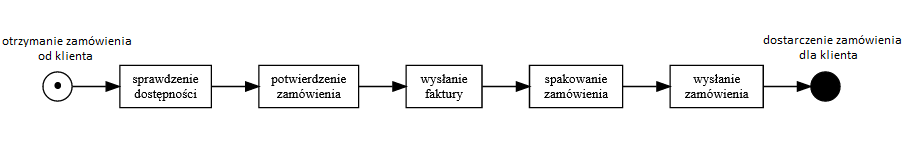
\includegraphics[scale=0.7]{simple-business-process.png}}
	\caption{\label{fig:simple_business_process}Przykład prostego procesu}
\end{figure}

Zauważmy, że mamy jasno zdefiniowany wejście - otrzymanie zamówienia od klienta oraz wyjście, kiedy dostarczamy oczekiwaną wartość dla klienta, a całość składa się z serii tworzących logiczną całość aktywności. Są one konkretnie zdefiniowane. Standardem jest zapisywanie aktywności w formie równoważników zdań.


\subsection{Zarządzanie procesami biznesowymi}
Zdefiniowanie procesu biznesowego otwiera wiele możliwości analizy działań przedsiębiorstwa i wskutek tego wprowadzanie usprawnień. Dziedziną, która się tym zajmuje, jest zarządzanie procesami biznesowymi (\textit{eng. Business process managment}) zwane w skrócie BPM. Sercem jest proces, a samo BPM jest dyscypliną używającą różnych metod, technik i sposobów w celu projektowania, wprowadzania w życie, zarządzania i analizy procesów biznesowych \cite{BPMDemystified}. 

Celem stosowania metod zarządzania procesami biznesowym jest udoskonalanie procesów w danej organizacji biznesowej. Udoskonalanie może być rozumiane w różnoraki sposób w zależności od kierunku rozwoju firmy. Może to być na przykład redukcja czasu, kosztów, czy dostarczanie lepszego produktu końcowego. Ważne jest, aby było to podejście całościowe i odnosiło się do całego zbioru aktywności w ramach danego procesu. Usprawnianie pojedynczej aktywności to nie jest BPM. Patrząc na przykład powyżej, jeśli wprowadzono by usprawnienia w ramach wysyłania faktury, robiąc to elektronicznie zamiast tradycyjną pocztą, mimo że taka zmiana przyniosłaby poprawę wydajności, nie byłoby to zarządzaniem procesami biznesowymi. O BPM można by mówić, gdyby znaleziono sposób, żeby przeprojektować cały proces tak, żeby wysyłanie faktury nie było potrzebne lub odwrotnie, jeśli dodano by nowe aktywności, co usprawniłoby proces jako całość czy nawet zmieniono kolejności zdarzeń w procesie, gdyż zmiana ilości poszczególnych, jednostkowych aktywności nie są konieczna, żeby ulepszyć proces jako całość \cite{BPMWhat}.

Zarządzanie procesami biznesowymi jest zbiorem praktyk, działań mających na celu udoskonalanie procesów. Trzeba więc rozumieć BPM jako pojęcie abstrakcyjne, jednak szczególnie w dzisiejszym świecie, zarządzanie procesami biznesowymi nie może się obyć bez wsparcia ze strony oprogramowania czy technik znanych z różnych dziedzin informatyki \cite{BPMSurvey}. Na lepsze zrozumienie czym zajmuje się zarządzanie procesami biznesowymi oraz w jaki sposób możemy zastosować informatykę, a w szczególności eksplorację procesów w tej dziedzinie, może pozwolić zrozumienie cyklu życia procesu biznesowego.

\begin{figure}[h]
	\centering{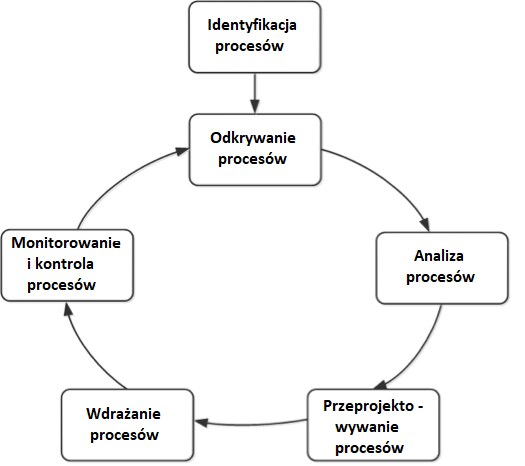
\includegraphics[scale=0.55]{lifecycle.png}}
	\caption{\label{fig:lifecycle}Cykl życia procesu biznesowego}
\end{figure}

Cykl życia procesu biznesowego (\textit{eng. Business process lifecycle}) przedstawiono na rys. \ref{fig:lifecycle} \cite{dumas2013fundamentals}. Jest to zbiór kroków niezbędnych do skutecznego zarządzania procesami biznesowymi. W celu dostosowania do zmieniającej się rzeczywistości poszczególne kroki powinny być co pewien czas powtarzane. 

Konieczność powtarzania elementów cyklu życia procesu biznesowego sygnalizuje przewagę komputerów i algorytmów nad wykonywaniem tych operacji przez człowieka. Metody informatyczne są stosowane, na każdym z wymienionych etapów. W szczególności dane zebrane w wyniku monitorowania procesów dają możliwość zastosowania metod z zakresu eksploracji procesów (sekcja \ref{sec:eksploracja}). Praca skupia się w głównej mierze na odkrywaniu procesów, czyli znajdowaniu istniejących już procesów na podstawie realnych danych. Należy zaznaczyć, że identyfikacja polega na ogólnym rozpoznaniu i nazwaniu zachodzących procesów, podczas gdy odkrywanie jest bardziej szczegółowe, a w jego wyniku otrzymujemy dokładny model.  

%---------------------------------------------------------------------------

\section{Eksploracja procesów}
\label{sec:eksploracja}
\subsection{Modelowanie procesów biznesowych}
\label{sec:modelling}
Na rys. \ref{fig:simple_business_process} przedstawiono przykład uproszczonego procesu biznesowego. Łatwo sobie wyobrazić, że proces ten w rzeczywistości może być znacznie bardziej skomplikowany. Część aktywności może być wykonywana równolegle, niektóre zdarzenia w ogóle nie zaistnieją lub będą występować kilkukrotnie w ramach jednego procesu. 

W sytuacji, w której zamówiony przez klienta towar będzie niedostępny, logiczne wydaje się poinformowanie go o opóźnieniu oraz danie mu możliwości anulowanie zamówienia lub jego kontynuacja i ponowne sprawdzenie dostępności. Ponadto, czynności takie jak wysłanie faktury oraz spakowanie i wysłanie zamówienia mogą być wykonane w dowolnej kolejności czy nawet jednocześnie przez dwie różne osoby. Proces staje się bardziej skomplikowany i konieczna do stworzenia jego modelu jest bardziej złożona notacja niż użyta do przedstawienia prostego procesu. 
Istnieje wiele notacji do modelowania procesów biznesowych, wśród nich można wymienić schematy blokowe, diagramy aktywności UML, łańcuchy procesu sterowanego zdarzeniami (\textit{eng. Event-driven Process Chains}), sieci Petriego \cite{BPMComparission}. Obecnie najpopularniejszą notacją używaną do opisu procesów biznesowych jest Business Process  Model and Notation, w skrócie BPMN \cite{omg2011bpmn}. Daje ona możliwość opisania w jednoznaczny sposób skomplikowanych procesów czy stworzenia diagramów współdziałania procesów, jednocześnie pozostając łatwą do zrozumienia.

Na grafice poniżej przedstawiono notację opartą o elementy BPMN, używaną w dalszej części pracy. Składają się na nią zdarzenia początkowe i końcowe, połączenia, bramki logiczne oraz aktywności. Czarnym kwadratem oznaczono sytuację, w której żadna aktywność nie jest wykonywana, co jest możliwe w bramce LUB. Także pętle mogą być pominięte, czyli wykonane zero razy.

\begin{figure}[H]
	\centering{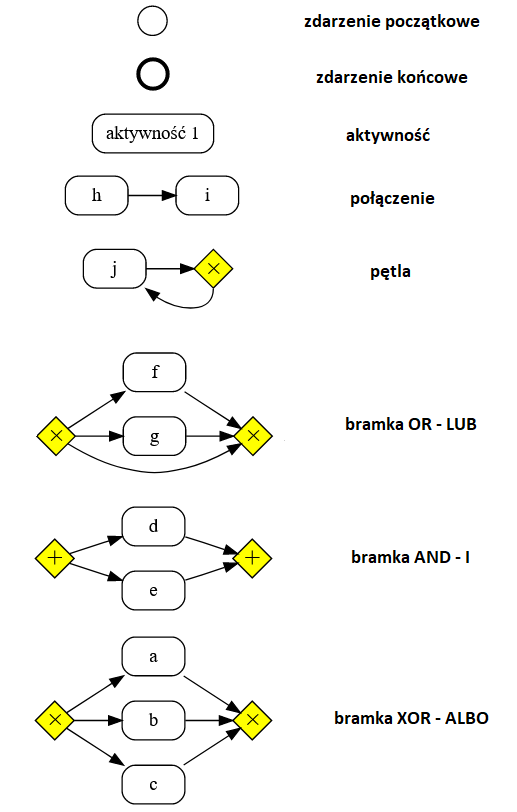
\includegraphics[scale=0.41]{BPMNelements.png}}
	\caption{\label{fig:bpmn_example}Elementy BPMN}
	\label{fig:lifecycle}
\end{figure}

Korzystając z tej notacji, można przedstawić opisany wcześniej proces. Na rys.  \ref{fig:complicated_business_process_1} widać model po modyfikacjach. 

\begin{figure}[h]
	\centering{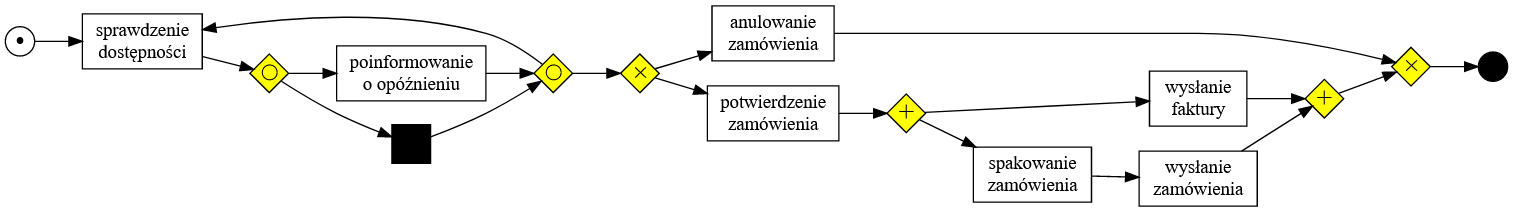
\includegraphics[scale=0.3]{complicated-process-example-1.png}}
	\caption{\label{fig:complicated_business_process_1}Rozbudowany model procesu - przykład 1}
\end{figure}

Możliwe jest teraz poinformowanie klienta o opóźnieniu, a następnie anulowanie zamówienia lub powtórne sprawdzenie dostępności. Model ten jednak nie jest wystarczająco precyzyjny i pozwala na potwierdzenie zamówienia po informacji o jego opóźnieniu, a bez uprzedniego ponownego sprawdzenia dostępności. Można zaproponować inny model (rys. \ref{fig:complicated_business_process_2}), który rozwiązuje powyższe problemy, jednak aktywność - poinformowanie o opóźnieniu - występuje w nim dwukrotnie, co jest niepożądane i pogarsza jego czytelność.

\begin{figure}[h]
	\centering{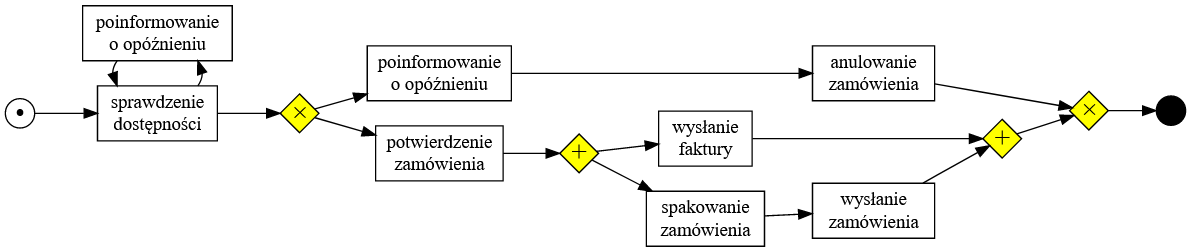
\includegraphics[scale=0.35]{complicated-process-example-2.png}}
	\caption{\label{fig:complicated_business_process_2}Rozbudowany model procesu - przykład 2}
\end{figure}

Co więcej, w pewnych przypadkach klient może mieć możliwość rezygnacji z zamówienia bez ówczesnego informowania go o opóźnieniu, a z czego nie zdawano sobie sprawy, wtedy konieczne może być stworzenie zupełnie innego modelu. Aby radzić sobie z tymi problemami, powstał szereg zestawów wytycznych, którymi warto się kierować, modelując procesy biznesowe. Wśród takich zasad można wymienić: zminimalizuj liczbę elementów w modelu, zminimalizuj liczbę ścieżek w modelu, używaj jednego zdarzenia początkowego i jednego końcowego, unikaj bramek LUB - OR , zdekomponuj model zawierający więcej niż 50 elementów \cite{7PMG}.

Modelowania procesów biznesowych jest próbą stworzenia uproszonej wersji rzeczywistości na podstawie przewidywań i założeń. Modele dają abstrakcję, użyteczne przybliżenie rzeczywistości, jednak należy pamiętać, że ,,Wszystkie modele są błędne'' i rzeczywisty proces najprawdopodobniej będzie różnił się od nawet najlepszego modelu. 


\subsection{Eksploracja procesów}

W dzisiejszych czasach standardem jest, że organizacje biznesowe korzystają z systemów informatycznych, takich jak, chociażby systemy ERP czy CRM, wspierających ich działalność. Systemy te rejestrują dane o procesach, które wspierają. Dane te mogą być później analizowane i wykorzystane do wprowadzenia usprawnień w działaniu firmy.   

Tradycyjne metody są wolne, kosztowne i narażone na błędy ludzkie, a konieczność ich ciągłego powtarzania, połączona z wszechobecnym w biznesie trendem automatyzacji sprawiają, że eksploracja procesów zyskuje na znaczeniu \cite{market-pm}. Ważna jest możliwość szybkiej adaptacji do zmian, a automatyzacja odkrywania procesów biznesowych pozwala na wykonywanie powtarzalnych zadań, eliminując przy tym błędy, co idealnie wpisuje się w ten trend.

Jest to szeroko pojęta dziedzina, która zawiera różne aplikacje inteligencji obliczeniowej, uczenia maszynowego i eksploracji danych do modelowania i analizy procesów. 
Jest wartościowym dodatkiem do innych metod eksploracji danych, gdyż zamiast skupiać się pojedynczym rezultacie i tworzyć dotyczące jego predykcje, celem jest zrozumienie całego procesu i akcji, które prowadzą do końcowego wyniku. Jest to trudniejsze, ale wyjątkowo cenne z punktu widzenia biznesowego, gdyż jakakolwiek zmiana w trakcie procesu może sprawić, że przewidywania będą kompletnie trafione, a zrozumienie całego procesu pozwala na pełniejszy obraz i łatwiejsze dostosowywanie się do zmian. 

Procesy biznesowe są zazwyczaj domeną analityków i menadżerów, którzy nie zawsze podchodzą do tematu ich analizy w sposób ścisły i mający odniesie w faktach, często opierając się na własnych przeczuciach czy doświadczeniach, wprowadzając czynnik ludzki, który może być przyczyną błędów. Metoda na stworzenie pomostu między metodami informatycznymi a biznesem i stworzenie możliwości na ścisłe, powtarzalne i sprawdzalne analizowanie procesów jest więc nad wyraz cenna. Eksploracja procesów biznesowych oparta jest bowiem na danych i nie ma w niej wiele miejsca na przypuszczenia i domysły.

Podsumowując, eksploracja procesów są to techniki, narzędzia oraz metody odkrywania, monitorowania i usprawniania rzeczywistych procesów poprzez wiedzę wyodrębnioną z dzienników zdarzeń powszechnie dostępnych w systemach informatycznych \cite{pm-manifesto}\cite{mining-overview}.
Wyróżnia się 3 podkategorie: 
\begin{itemize}
  \item[•] automatyczne odkrywanie procesów
  \item[•] sprawdzanie zgodności (\textit{eng. conformance checking})
  \item[•] udoskonalanie procesu (\textit{eng. performance mining})
\end{itemize}


\subsection{Dzienniki zdarzeń}
\label{sec:event_logs}
Danymi wejściowymi dla algorytmów z dziedziny eksploracji procesów są dzienniki zdarzeń, zwane często logami.
 
\begin{figure}[h]
	\centering{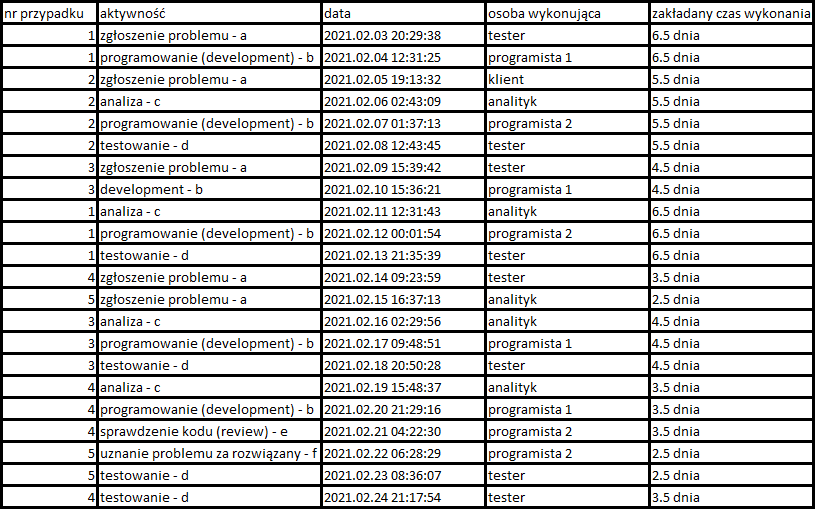
\includegraphics[scale=0.6]{event-log-example.png}}
	\caption{\label{fig:event_log_example}Przykład dziennika zdarzeń}
\end{figure}

Przyjmuje się, że aby mówić o dzienniku zdarzeń powinien on zawierać 3 informacje: numer przypadku, czyli unikalny identyfikator zbioru aktywności, nazwę aktywności oraz datę jej wykonania - ważną tylko w kontekście kolejności wykonywania pojedynczych aktywności. Ponadto może on zawiera inne zbędne w kontekście odkrywania procesów biznesowych dodatkowe informacje, takie jak: podmiot wykonującym daną aktywność, miejsce, koszt czy aktualny postęp wykonania. Oczywiście te pozostałe dane mogą być wykorzystywane w kolejnych etapach analizy i usprawniania procesu.

Mając do dyspozycji te 3 informacje - poszczególne przypadki, aktywności na nie się składające oraz ich kolejność, zliczane jest, jak często poszczególne aktywności występują w danej kolejności. Każdy taki przypadek zwany jest wariantem procesu. Oprócz tego niezbędna jest wiedza, jak często dany wariant wystąpił.

\begin{figure}[h]
	\centering{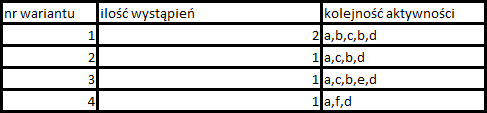
\includegraphics[scale=0.6]{variants-example.png}}
	\caption{\label{fig:process_variants_example}Warianty procesu odpowiadające przykładowemu dziennikowi zdarzeń}
\end{figure}

Dla poprawy czytelności aktywności często reprezentowane są jako symbole, np. kolejne litery alfabetu, zamiast pełnej nazwy.

\subsection{Automatyczne odkrywanie procesów biznesowych}
\label{sec:discovery}

Automatyczne odkrywanie procesów biznesowych jest poddziedziną eksploracji procesów i obejmuje techniki przekształcania danych w procesy. Ważne, że proces już istnieje i jest on jedynie odkrywany. Wejściem jest dziennik zdarzeń, a wyjściem mapa lub model procesu.

Zaprojektowane procesy nie zawsze są realizowane w praktyce. Ważne jest, żeby proces był oparty na analizie prawdziwych danych, a nie spekulacjach i założeniach. Pozwala na znajdowanie procesu takim, jaki jest, a nie takim, jakim chciano by, żeby był.

\begin{figure}[h]
	\centering{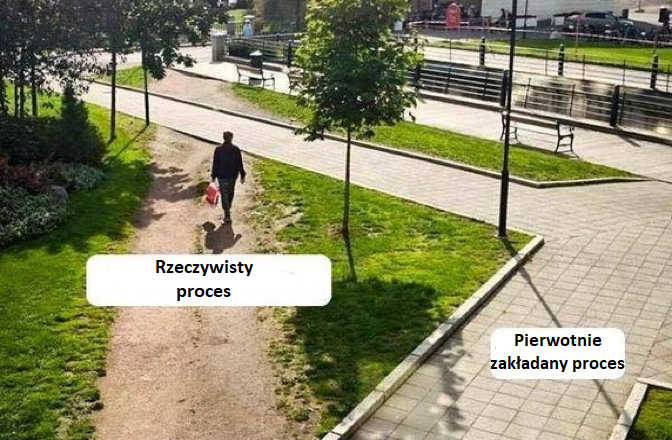
\includegraphics[scale=0.5]{model-vs-real.png}}
	\caption{\label{fig:subcaption_example}Proces rzeczywisty i pierwotnie zakładany}
\end{figure}

Celem automatycznego odkrywania procesów biznesowych jest zaprojektowanie funkcji - algorytmu, która przekształci dane z dziennika zdarzeń w model procesu \cite{pm-book}. Istnieje wiele algorytmów do odkrywania procesów biznesowych. Wśród najpopularniejszych można wymienić:
\begin{itemize}
  \item[•] Alpha algorithm \cite{alpha-algorithm}
  \item[•] The ILP Miner \cite{ILP-miner}
  \item[•] Heuristic Miner \cite{heuristics-miner}
  \item[•] Multi-phase Miner \cite{multi-phase-miner}
  \item[•] Inductive Miner \cite{inductive-miner}
\end{itemize}

Istnieją 4 powszechnie używane kryteria do określania jakości otrzymanego model. Są to:
\begin{itemize}
  \item[•] odwzorowanie (\textit{eng. fitness}) - zgodność modelu z dziennikiem zdarzeń.
  \item[•] prostota (\textit{eng. simplicity}) - złożoność i łatwość zrozumienia modelu.
  \item[•] precyzja (\textit{eng. precision}) - brak zachowań niezwiązanych z logiem, a możliwych w modelu.
  \item[•] generalizacja (\textit{eng. genralization}) - odzwierciedlenie w modelu prawdopodobnych aktywności, mimo że nie znajdują się one w logu.
\end{itemize}
Konieczne jest znalezienie balansu między nimi, gdyż często starając się poprawiać model pod kątem jednego kryterium, pogorszy się on pod względem innych. Powstało wiele metryk przedstawiających te kryteria za pomocą wzorów matematycznych \cite{conf-propositions} \cite{Blum2015MetricsIP}.
Bardziej szczegółowo wybór metryk omówiono w sekcji \ref{sec:metryki}.

Wśród problemów dotykających istniejące algorytmy można wymienić problem ze znajdowaniem aktywności zachodzących równolegle, brak możliwości pomijania aktywności czy reprezentowania duplikatów, nieradzenie sobie z zakłóceniami w logu, tworzenie zbyt skomplikowanych modeli, czy trudność z odwzorowaniem niektórych zachowań. Modele stworzone mogą nie być spójne strukturalnie \cite{dongen2006b} \cite{StructuralDetectionofDeadlocks}, przez co rozumie się modele, w których istnieje aktywność, z której nie możemy osiągnąć zdarzenia końcowego lub nie może być ona w żaden sposób osiągnięta ze zdarzenia początkowego. Metody te zazwyczaj oparte są na grafach bezpośrednich następstw (\textit{eng. directly follows graphs}), przez co problemem może być sytuacja, kiedy log jest niekompletny. 

Zastosowanie algorytmów genetycznych do automatycznego odkrywania procesów biznesowych może być odpowiedzią na te kłopoty. Takie podejście pozwala na wyeliminowanie części problemów często dotyczących innych metod. Najważniejszą jednak przewagą algorytmów genetycznych jest pełna dowolność w kwestii generowania modelu pod kątem metryk zdefiniowanych przez użytkownika. Często znalezienie dobrze dopasowanego do logu modelu może być okupione stworzeniem bardzo skomplikowanego modelu - niewystarczająca prostota, pozwalającego na wiele zachowań nieobecnych w logu - niewystarczająca precyzja. Algorytm ewolucyjny pozwala na nieograniczoną możliwość manipulacji parametrami, żeby znaleźć oczekiwany balans między wszystkimi metrykami. Możliwe jest też stworzenie nowych, własnych metryk, gdyż są one niezależne od samego algorytmu ewolucyjnego. Klasyczne algorytmy mają problem z uzyskaniem dobrych rezultatów dla wszystkich metryk i nie mają możliwości zmiany parametrów startowych.

%---------------------------------------------------------------------------

\section{Ewolucja gramatyczna}
\label{sec:ewolucjaGramatyczna}
\subsection{Algorytmy ewolucyjne}
Algorytmy ewolucyjne \cite{EA} są inspirowaną selekcją naturalną metaheurystyką, która używa znanych z ewolucji biologicznej operacji jak selekcja, krzyżowanie czy mutacja do rozwiązywania problemów wyszukiwania i optymalizacji. Są rodziną metod przeszukiwania przestrzeni losowych rozwiązań w celu wyszukania najlepszych z nich. 

Algorytmy ewolucyjne znajdują zastosowanie w problemach, dla których nie jest konieczna gwarancja znalezienia najlepszego rozwiązania. Cechami wyróżniającymi je na tle innych algorytmów uczenia maszynowego jest istnienie puli zamiast jednego rozwiązywania, co umożliwia szersze przeszukiwanie przestrzeni rozwiązań oraz nieograniczoną i łatwą w zaimplementowaniu paralelizację. Algorytmy te są znacznie bardziej nastawione na globalne eksplorowanie nowych rozwiązań, zamiast na jak najszybsze osiągnięcie celu. Z tego względu dobrze nadają się do problemów, gdzie istnieje dużo ekstremów, a przestrzeń poszukiwań jest duża. Jako przeciwieństwo, metody oparte na gradiencie w najprostszej znajdują tylko lokalne ekstrema, nawet po modyfikacjach takich, jak na przykład simulated anneling wciąż nie ma populacji i możliwości tak szerokiego przeszukiwania przestrzeni rozwiązań.

Sposób działania algorytmów genetycznych polega na stworzeniu populacji losowych rozwiązań zwanych genotypami lub chromosomami, które kodowane są za pomocą genów reprezentowanych przez bity, liczby lub znaki i zapisywanych w strukturze łatwo przetwarzalnej przez komputer. Najczęściej jest to lista jednowymiarowa liczb całkowitych. Fenotyp natomiast jest reprezentacją utożsamianą z docelowym programem lub modelem. Genotyp może być równoznaczny z fenotypem, jednak poza prostymi przykładami, zazwyczaj są to oddzielne reprezentacje i geny mapowane są na odpowiadające wartości w fenotypie, zwane allelami. Fenotyp jest postacią, dla której możliwe jest obliczanie funkcji dopasowania (\textit{eng. fitness function}), co pozwala ocenić, jak dobre jest wygenerowane rozwiązanie. Następnie, istniejąca populacja jest modyfikowana poprzez krzyżowanie i mutacje. Warto zauważyć, że krzyżowanie przeszukuje przestrzeń rozwiązań globalnie, podczas gdy mutacja odpowiada za lokalne wyszukiwanie. Po zastosowaniu tych operatorów i sklasyfikowaniu rozwiązań, spośród głównie, choć nie tylko najlepszych osobników, utworzona zostaje nowa populacja, dla której cały proces jest powtarzany do momentu znalezienia satysfakcjonującego rezultatu.

\subsection{Szczegółowe omówienie operatorów i działania algorytmów ewolucyjnych}
Tworzenie populacja jest pierwszym krokiem algorytmu ewolucyjnego. Może ono odbywać się kompletnie losowe lub do tworzenia nowych osobników może zostać użyta odpowiednia heurystyka. 

Kolejny krok - selekcja - pozwala na zachowanie w populacji części osobników promując najlepszych z nich, co sprawia, że przeszukiwanie przestrzeni rozwiązań nie jest kompletnie losowe. Można skorzystać z metod takich jak:
\begin{itemize}
  \item[•] Selekcja proporcjonalna - wybierane są losowo osobniki z puli wszystkich populacji z warunkiem, że rozwiązania z największą wartością metryk mają większą szansę na bycie zachowanymi w populacji. 
  \item[•] Selekcja turniejowa - wybierany jest podzbiór ze zbioru rozwiązań i zachowywane w przyszłej populacji są najlepsze osobniki z tego podzbioru. Rozwiązanie to pozwala na duży wpływ na presję genetyczną - zwiększając wielkość podzbioru, ograniczamy szansę na wybór z niską wartością metryk. Jest to metoda łatwa w implementacji, która umożliwia łatwe zrównoleglenie.
\end{itemize}

Żeby uniknąć sytuacji, w której najlepsze rozwiązania zostaną zmodyfikowane, możliwe jest zastosowanie elityzmu, który pozwala na zachowanie w kolejnej generacji części najlepszych osobników w populacji niezależnie od wyniku selekcji.

Następnie stosowane są operatory krzyżowania i mutacji. Krzyżowanie jest zamianą materiału genetycznego, czyli części genotypu pomiędzy dwoma osobnikami w populacji tworząc również dwa zmienione osobniku. Mutacja natomiast zachodzi w obrębie jednego osobnika.

\begin{figure}[h]
	\centering{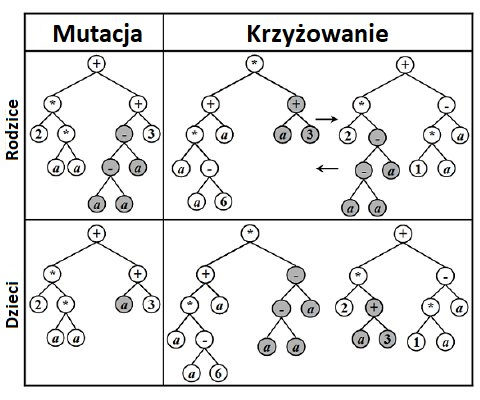
\includegraphics[scale=0.6]{Mutation-and-crossover-operations.jpg}}
	\caption{\label{fig:mutation-and-crossover-operations}Mutacja i krzyżowanie}
\end{figure}

Operatory te nie muszą i zazwyczaj nie są stosowane do każdego osobnika w populacji, a to jak często powinny być stosowane, ustalane jest za pomocą odpowiedniego parametru. Zdarza się, że mutacja jest stosowana więcej niż dla danego genu w danym genotypie.

Najczęściej używane operatory krzyżowania to:
\begin{itemize}
\item[•] Krzyżowanie punktowe - spośród dwóch genotypów losowo wybierany jest jeden punkt, następnie tworzone są dwa nowe genotypy pierwszy z genów na prawo od punktu w pierwszym genotypie i na lewo w genotypie drugim oraz drugi z dwóch pozostałych.

\item[•] Krzyżowanie dwupunktowe - spośród dwóch genotypów losowo wybierane są dwa punkty, następnie część pomiędzy tymi punktami jest zamieniana pomiędzy genotypami.

\item[•] Krzyżowanie n-punktowe - uogólnienie powyższych krzyżowań dla n punktów.

\item[•] Krzyżowanie zamiana w drzewie - metoda opiera się na modyfikacjach w fenotypie, który jest reprezentowany jako drzewo, w tej metodzie zamieniane są ze sobą dwa poddrzewa. W tym przypadku tworzone są tylko prawidłowe rozwiązania, jednak jest to metoda wymagająca większej ilości obliczeń.  
\end{itemize}
Ponadto krzyżowania możemy podzielić na stało-punktowe, czyli takie, w którym wybierany jest ten sam punktu lub punkty w obu osobnikach, przez co nowe genotypy mieć tą samą długość jak rodzice i zmienno-punktowe, gdzie mogą to być różne punkty, co skutkuje dużą zmienności w rozmiarach utworzonych genotypów. 

Natomiast operatory mutacji to:
\begin{itemize}
\item[•] Mutacja punkowa - dowolny gen w genotypie zostaje zmieniony na inną losową wartość. Przez co odpowiadająca mu produkcja tworzy nową wartość. Pozostałe produkcje pozostają niezmienione.

\item[•] Mutacja zamiana w drzewie - metoda opiera się modyfikacjach w fenotypie, który jest reprezentowany jako drzewo, w tej metodzie tworzone jest nowe poddrzewo. Analogicznie jak w przypadku krzyżowania tworzone są tylko prawidłowe rozwiązania, jednak konieczna jest większa ilość obliczeń. 
\end{itemize}

Ostatnim krokiem jest zastąpienie osobników w poprzedniej populacji przez nowych powstałych na skutek zastosowania wcześniej wspomnianych operatorów. Istnieją dwa podejścia, sugerujące zastępowanie całej populacji lub tylko kilku osobników \cite{SSvsGen}.


\subsection{Ewolucja gramatyczna}
Optymalny model procesu biznesowego może mieć różną długość, dlatego chcąc znaleźć taki model, potrzebujemy metody, która pozwoli na generowanie rozwiązań o zmiennej długości. Tradycyjne algorytmy genetyczne operują na stałej strukturze i mogą być użyte na przykład, żeby dobrać odpowiednie parametry do istniejącego modelu. W wielu problemach jednak chcemy rozwiązanie o nieznanym rozmiarze, dlatego obecnie najpopularniejsza metoda to programowanie genetyczne \cite{Koza:1990:pat-GAsp}\cite{10.5555/138936}, które pozwala na generowanie rozwiązań o różnym rozmiarze, dzięki ewolucji całej struktury fenotyp, najczęściej reprezentowane jako drzewo. Najczęściej te są gotowymi wykonywalnymi programami, jednak mogą być też równaniami czy modelami.

Oparta na programowaniu genetycznym jest ewolucja genetyczna \cite{ryan_collins_neill_1998}. Korzysta ona ze standardowych metod ewolucji genetycznej, jednak ewoluuje gramatykę w celu znalezienia programu, który najlepiej rozwiązuje problem. Gramatyka najczęściej zapisana w notacji BNF (sekcja \ref{sec:BNF}). Dzięki zastosowaniu rekursywnych produkcji możliwe jest tworzenie rozwiązań o różnej długości. 

\subsection{BNF}
\label{sec:BNF}
Gramatyka jest zbiorem zasad opisujących budowę języka. Opisuje syntaktykę języka, czyli sposób łączenia poszczególnych symboli, nie mówiąc nic o znaczeniu poszczególnych słów języka. Odnosi się to także do języków formalnych np. języków programowania. Do opisu takich języków służą gramatyki formalne. Na gramatykę formalną składa się z uporządkowana czwórka G = (T,N,P,S), gdzie 

\begin{itemize}
  \item[•] T - skończony zbiór symboli terminalnych, czyli stałych, symboli, które nie mogą być zastąpione innym ani podzielone na mniejsze 
  \item[•] N - skończony zbiór symboli nieterminalnych, czyli zmiennych, symboli, które są modyfikowane przy tworzeniu języka
  \item[•] P - skończony zbiór produkcji, czyli zasad, przekształceń postaci (N$\cup$T)*N(N$\cup$T)* -> (N$\cup$T)*, czyli przynajmniej jednego symbolu nieterminalnego w dowolny zbiór symboli terminalnych i nieterminalnych.
  \item[•] S - symbol startowy, gdzie S $\in$ N
\end{itemize}

W informatyce szczególnie szeroko stosowane są gramatyki bezkontekstowe. Pozwalają one na pokazanie, w jaki sposób rekurencyjnie tworzony jest język, co jest potrzebne, żeby zrozumieć znaczenie programu. Zaletą jest też ich stosunkowo łatwe parsowanie.
Gramatyka bezkontekstowa jest to gramatyka, w której wszystkie produkcje mają postać:
\begin{center}
	A -> {$\alpha$},
\end{center}
gdzie A jest to pojedynczy symbol nieterminalny, a $\alpha$ to dowolny zbiór symboli terminalnych i nieterminalnych.
	
Notacja Backusa-Naura (\textit{eng. Backus-Naur Form}) \cite{Backus1959TheSA}\cite{Naur}\cite{Knuth1964} jest najpopularniejszą notacją używaną do kodowania gramatyk bezkontekstowych. Symbole, które składają się na BNF to:

\begin{itemize}
  \item[•] ::= - produkcja
  \item[•] |   - lub
  \item[•] <>  - symbole nieterminalne
\end{itemize}

Używając tych symboli, możemy opisywać składnie języka w następujący sposób:
\begin{center}
<Nieterminalny1> ::= <Nieterminalny2>Terminany1 | <Nieterminalny3> | Terminany1
\end{center}
Oczywiście możliwe jest też definiowanie rekurencyjnie, co pozwala na tworzenie skomplikowanego języka za pomocą prostych zasad: 
\begin{center}
<Nieterminalny1> ::= <Nieterminalny2> | <Nieterminalny2><Nieterminalny1>
\end{center}

\subsection{Tworzenie gramatyki pod kątem ewolucji}
\label{grammarCreation}
Dla każdego problemu można stworzyć nieskończoną ilość poprawnych gramatyk, jednak nie wszystkie z nich będą odpowiednie do zastosowania w algorytmie ewolucji gramatycznej. Chcąc stworzyć gramatykę, która umożliwi najwydajniejsze rozwiązanie problemu można przyjąć kilka wytycznych \cite{grammarDesign}: 
\begin{itemize}
  \item[•] Każda rekursywna produkcja powinna mieć co najmniej tyle samo produkcji nierekursywnych, inaczej biorąc pod uwagę, że genotyp jest mapowany na fenotyp metodą pseudolosową, prawdopodobieństwo otrzymania rozwiązania, które musi się składać tylko symboli terminalnych, będzie zbyt niskie.
  \item[•] Tworząc gramatykę pod kątem wykorzystania jej w procesie ewolucji, ważne jest, żeby ilość produkcji jak najlepiej odzwierciedlała, jak często chcemy uzyskać dane rozwiązanie.
  \item[•] Stosując mutacje oraz krzyżowanie punktowe lub n-punktowe, które jak wiadomo, podmienia geny w genotypie, może dojść do sytuacji, w której dany gen po podmianie zostanie zmapowany na produkcje o innej ilości symboli nieterminalnych, przez co kolejne geny, będą mapowania niezgodnie z pierwotnym sensem, gdyż ilość genów w genomie pozostaje stała. Żeby temu zapobiec, należy ograniczyć ilość symboli nieterminalnych do minimum, a każdy symbol nieterminalny powinien mieć produkcje tworzące tyle samo symboli nieterminalnych oraz możliwie tyle samo produkcji, dzięki czemu po zmapowaniu symbole nadal będą odpowiadały pierwotnym. 
  \item[•] Stworzona gramatyka powinna umożliwić na tworzenie jak najmniejszej ilości rozwiązań, które nie należą do języka, co prawda nie uniemożliwi to działania algorytmu, gdyż można odrzucić te rozwiązania na etapie parsowania, ale warto oszczędzić niepotrzebnych obliczeń i rozwiązań ten problem już na etapie tworzenia gramatyki. 
\end{itemize}

\subsection{Omówienia działania algorytmu ewolucji genetycznej}
Mechanizmem, który wyróżnia ewolucji genetyczną na tle innych algorytmów ewolucyjnych, jest mapowanie genotypu zapisywanego jako jednowymiarowa tablica liczb całkowitych na fenotyp - język, zgodnie z zasadami stworzonej gramatyki. Przykładem może być genotyp: 
\begin{center} [6, 71, 92, 59, 52, 95, 23, 45, 12, 2] \end{center}
i gramatyka w notacji BNF:

 \begin{center}
  \begin{tabular}{l}
    <e> ::= <var>=<math><var> \\
	<math> ::= <math><math> | <var><op> \\
	<op> ::= + | - \\
	<var> ::= a | b | c | d,
  \end{tabular}
 \end{center}

której symbolem startowym jest <e>. 
Wybór kolejnych produkcji odbywa się według zasady:
\begin{center} $produckja = gen\_jako\_liczba\_całkowita\ \%\ ilosc\_dostepnych\_produkcji$ \end{center}
Używając wyprowadzenia lewostronnego:

\begin{itemize}
  \item[•] Aktualne wyrażenie: <e>; \newline
Aktualny symbol nieterminalny: <e>; \newline
Ilość możliwych produkcji: 1; \newline
Wartość genu: 6; \newline
6 mod 1 = 0, więc <e> zostaje zastąpiony przez <var>=<math><var>
  \item[•] Aktualne wyrażenie: <var>=<math><var>; \newline
Aktualny symbol nieterminalny: <var>; \newline
Ilość możliwych produkcji: 4; \newline
Wartość genu: 71; \newline
71 mod 4 = 3, więc <var> zostaje zastąpiony przez d
  \item[•] Aktualne wyrażenie: d=<math><var>; \newline
Aktualny symbol nieterminalny: <math>; \newline
Ilość możliwych produkcji: 2; \newline
Wartość genu: 92; \newline
92 mod 2 = 0, więc <math> zostaje zastąpiony <math><math>
  \item[•] Aktualne wyrażenie: d=<math><math><var>; \newline
Aktualny symbol nieterminalny: <math>; \newline
Ilość możliwych produkcji: 2; \newline
Wartość genu: 59; \newline
59 mod 2 = 1, więc <math> zostaje zastąpiony <var><op>
\end{itemize}
Kontynuując analogicznie, po zastąpienie wszystkich symboli nieterminalnych, ostatecznie otrzymany fenotyp to:
\begin{center} d = a - b + c \end{center}	
Używanie tego prostego mechanizmu, w przypadku bardziej skomplikowanej gramatyki, możliwe jest generowanie znaczniej bardziej złożonych rozwiązania. W połączeniu z metodami z algorytmów ewolucyjnych możliwe jest teoretycznie ewoluowanie programów w dowolnym języku programowania, a następnie za pomocą odpowiedniej funkcji dopasowania znalezienie takiego, który rozwiąże dany problem. W kolejnej sekcji omówiono jak dobrać metryki, aby użyć tego mechanizmu do odkrywania procesów biznesowych.


%---------------------------------------------------------------------------

\section{Metryki}
\label{sec:metryki}

\subsection{Metryki a funkcja dopasowania}

Funkcja dopasowania jest obliczana w każdej iteracji, dla każdego osobnika w populacji, dlatego powinna być możliwie najmniej kosztowna obliczeniowo. Nie warto więc nadmiernie jej komplikować, gdyż nawet jeśli taka wersja lepiej określi, jak dobre jest dane rozwiązanie, to jej obliczenie, może stać się wąskim gardłem całego algorytmu, co poprzez zwiększenie czasu potrzebnego na znalezienie rozwiązania pogorszy jego działanie. 

Dobierając funkcje dopasowania, ważne jest, że była ona regularna, gdyż duża ilość lokalnych ekstremów może spowolnić ewolucję, a nawet całkowicie uniemożliwić znalezienie globalnie najlepszego rozwiązania.
Nie może więc ona jedynie bezwzględnie mierzyć, jak dobre jest rozwiązanie. Dobry przykładem jest tutaj problem układanie planów (\textit eng. timetabling problem), gdzie większość otrzymanych rozwiązań będzie nieprawidłowa, a fitness będzie wynosił zero, nawet jeśli mała zmiana może sprawić, że znalezione zostanie właściwe rozwiązanie, dlatego konieczne jest, jak najlepsze uchwycenie jak blisko algorytm jest prawidłowego rozwiązania \cite{icga85:cramer} \cite{beasley:1993:ogapf}.

Ostatecznie funkcja dopasowania w naszym algorytmie jest średnią ważoną metryk wymienionych w sekcji \ref{sec:discovery}, jednak oprócz tego dodano kolejną metrykę złożoność, która ma poprawiać funkcje dopasowania zgodnie z powyższymi zasadami. Użytkownik może określić, z jakimi wagami wziąć pod uwagę poszczególne metryki.

\subsection{Dodatkowa metryka - złożoność}
\label{sec:additional-metric-complexity}
Dodatkowa metryka zawiera informacje niedotyczące bezpośrednio jakości odkrytego modelu. Istnieją jednak  teoretyczne przesłanki, że powinna wpłynąć pozytywnie na działanie algorytmu. W odróżnieniu od innych metryk celem jej używania jest poprawa wydajności algorytmu ewolucji i próba zminimalizowania czasu potrzebnego na znalezienie rozwiązania.
 
Zamysłem jest promowanie rozwiązywania prostych problemów w prosty sposób i unikanie lokalnych ekstremów - w tym wypadku sytuacji, w której populacja zostanie zdominowana przez zbyt skomplikowane osobniki na wczesnym etapie ewolucji, zamiast tego ewolucja jest bardziej nakierowana na znajdowanie coraz lepszego rozwiązania wraz ze wzrostem stopnia skomplikowania modelu. Analogię można odnaleźć w naturze, w pewnym momencie na Ziemii dinozaury były najlepiej przystosowanymi do życia na tej planecie organizmami - lokalne maksimum i blokowały powstawanie mniej skomplikowanych form życia, jednak jak pokazuje historia, po wyginięciu dinozaurów, te były w stanie stać się jeszcze lepiej przystosowanymi istotami.

Większa złożoność każdego modelu przekłada się także na dłuższe obliczanie metryk dla niego, przez co znalezienie ostatecznego rozwiązania zajmuje więcej czasu.

Kolejną zaletą jest to, że złożoność korzysta z istniejących już obliczeń, przez co nie zwiększa w istotny sposób czasu każdej iteracji algorytmu, co dodatkowo pozwala na łatwiejsze porównanie działania algorytmu z i bez tej metryki.

\subsection{Metryki - szczegóły}
\label{sec:metrics-details}
\subsubsection{Prostota}  
Jest to najprostsza z metryk. Celem jest zmniejszenie skomplikowania modelu. Głównym czynnikiem na to wpływającym jest ilość aktywności w modelu. Idealna byłaby sytuacja, w której model ma tyle samo aktywności, ile unikalnych aktywności jest w dzienniku zdarzeń. To nie zawsze jest możliwe, jednak chcąc otrzymać maksymalnie czytelny model, powinniśmy do tego dążyć. Stąd też metryk wybrana skupia się na dwóch czynnikach, czyli ilości duplikatów w modelu i ilości brakujących wartości w modelu. Oczywiście znaczenie ma wielkość modelu, dlatego wartości tego musimy odnieść do ilości wszystkich zdarzeń w logu i modelu. Metrykę zapożyczono z \cite{qd-in-discovery} i ostatecznie wyrażono wzorem: \begin{center}
$M_{pro} = 1 - \frac{ilosc\ duplikatow\ w\ modelu\ +\ ilosc\ brakujacych\ zdarzen\ w\ modelu}{ilosc\ unikalnych\ zdarzen\ w\ logu\ +\ ilosc\ zdarzen\ w\ modelu}$
\end{center}
\subsubsection{Odwzorowanie} 
Jest to najbardziej kosztowna obliczeniowo metryka. Pozostałe metryki obliczane są na podstawie informacji uzyskanych podczas jej obliczania. Ważne jest, żeby obliczać dopasowanie częściowo dla każdej aktywności, a nie całego wariantu procesu, co sprawi, że metryka będzie bardziej wrażliwa na zmiany. Możliwe jest zastosowanie prostej zero-jedynkowej metryki do obliczania, która weryfikowałaby czy model całkowicie zgadza się z wariantem logu, jednak co jest szczególnie niekorzystne w przypadku algorytmu genetycznego, nie byłoby sprawdzane, o ile bliżej jesteśmy do celu, dopóki losowo nieznaleziony zostałby model idealnie pasujący do wariantu. Metrykę oparto o \cite{metric-calculation}, jednak przy procesie z wieloma aktywnościami, najczęściej części aktywności może zostać dopasowana, co sprawi, że łączny błąd będzie niewielki, dlatego wprowadzono modyfikację i podniesiono otrzymany wynik do potęgi 4, żeby zrobić metrykę bardziej wrażliwą na zmiany. Ostatecznie metrykę wyrażono wzorem:
\begin{center}
\begin{tabular}{l}
$M_o = (1 - blad\_odwzorowania)^4$ \\
$blad\_odwzorowania = \frac{\sum_{ilosc\ procesow\ w\ logu} \frac{blad\ odwzorowania\ logu\ w\ modelu}{minimalna\ długosc\ najlepszej\ sciezki\ w\ modelu\ +\ długosc\ sciezki\ w\ logu}}{ilosc\ zdarzen \ w\ logu}$
\end{tabular}
\end{center}
\subsubsection{Precyzja} 
Pozwala na unikanie niewystarczającego dopasowania (\textit{eng. underfitting}). Celem jest uniknięcie tworzenia modeli, według których możliwe są praktycznie dowolne zachowania. Możliwe jest osiągnięcie maksymalnej wartości pozostałych metryk, tworząc jednak bramkę LUB - OR zawierającą wszystkie aktywności, jednak oczywiste jest, że nie jest to pożądany model. We wzorze skupiono się na ilości osiągalnych zdarzeń następujących po danej aktywności, możliwych w modelu. Chcemy, żeby poszczególne aktywności mogły poprzedzać tylko te, które rzeczywiście poprzedzają w logu. Metrykę oparto o \cite{precision-calculation}, jednak otrzymany wynik podniesiono do potęgi $\frac{1}{3}$, bo oryginalna metryka jest zbyt wrażliwa na zmiany, przez co jest nieproporcjonalna do innych, co zwiększa prawdopodobieństwo utknięcia w lokalnym maksimum, gdzie każda mała zmiana w modelu będzie powodować ogromną zmianę w metryce. Ostatecznie wyrażono ją wzorem:
\begin{center}
$M_{pre} = (1 - \sum_{zdarzenia\ w\ modelu} \frac{ilosc\ osiagalnych\ zdarzen\ w\ modelu\ -\ ilosc\ osiagalnych\ zdarzen\ w\ logu}{ilosc\ osiagalnych\ zdarzen\ w\ modelu})^{\frac{1}{3}} $
\end{center}
\subsubsection{Generalizacja}
Pozwala na unikanie nadmiernego dopasowania (\textit{eng. overfitting}). W pierwszej chwili może wydawać się przeciwieństwem precyzji, jednak chodzi tutaj o uwzględnienie brakujących w dzienniku zdarzeń wariantów, a nie o rozszerzenie modelu o nowe, zupełnie niezwiązane z istniejącymi. Dobrą wizualizacją jej działania jest operacja domknięcia znana z dziedziny przetwarzania obrazów cyfrowych. Generalizację można zmierzyć poprzez obliczenie średniej ważonej liczby przejść w modelu przez dane zdarzenie, dzięki czemu wciąż uwzględniane są ścieżki, które są często odwiedzane w innych wariantach, mimo że pozwalają na zachowanie niewidoczne w dzienniku zdarzeń, a jednocześnie karane jest istnienie ścieżek, które zupełnie nie pokrywają się z żadnymi wariantami. Wraz ze zwiększaniem ilości wykonań danej aktywności wzrasta pewność, że ścieżki ją uwzględniające faktycznie istnieją i ta informacja staje się mniej cenna, dlatego wzięto pierwiastek z liczby wystąpień danego zdarzenia. Metrykę zapożyczono z \cite{qd-in-discovery} i ostatecznie wyrażono wzorem:
\begin{center}
$M_g = 1 - \frac{\sum_{zdarzenia\ w\ modelu} \frac{1}{\sqrt{ilosc\ wystapien\ zdarzenia}}}{ilosc\ zdarzen\ w\ logu} $
\end{center}
\subsubsection{Złożoność}
Metryka jest powiązana z odwzorowaniem. Jeśli odwzorowanie rośnie, pozwalamy na tworzenie bardziej skomplikowanego modelu. Złożoność jest wyrażana jako ilość wszystkich możliwych ścieżek w modelu. W przypadku pętli złożoność byłaby nieskończona, dlatego przyjęto, że pętla oznacza maksymalnie dwukrotne wykonanie pętli. Jako że np. dla bramki AND jest to n!, zauważamy, że złożoność rośnie niewspółmiernie szybciej do odwzorowania, dlatego we wzorze wzięto pierwiastek ze złożoności. Ostatecznie metrykę wyrażono wzorem: 
\begin{center}
$M_z = 1 - \frac{1}{\sqrt{1\ +\ blad\_odwzorowania\ *\ \sqrt{zlozonosc\ modelu}}} $
\end{center}
\subsection{Obliczanie metryk}
W sekcji \ref{sec:event_logs} przedstawiono przykład dziennika zdarzeń i warianty procesu uzyskane z niego. Poniżej przedstawiono, jak mógłby wyglądać model tego procesu - na czerwono zaznaczono ilość wykonań danej aktywności - oraz zademonstrowano obliczanie metryk:

\begin{figure}[h]
	\centering{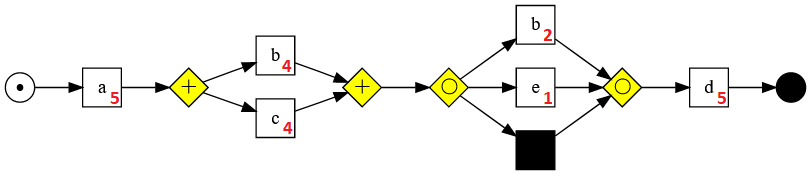
\includegraphics[scale=0.5]{model-metrics.png}}
	\caption{\label{fig:metrics_business_process}Model, dla którego obliczane są metryki}
\end{figure}

\subsubsection{Obliczanie prostoty}
Model posiada jest jeden duplikat - \textbf{b} oraz jedno brakujące zdarzenie - \textbf{f}, więc wartość metryki wynosi:
\begin{center}
$M_{pro} = 1 - \frac{1\ +\ 1}{6\ +\ 6} = 0.8333$
\end{center}

\subsubsection{Obliczanie odwzorowania}
\label{sec:alignment-calculation}
Są trzy możliwość na niezgodność modelu z logiem -  brak zdarzenia w modelu, brak zdarzenia w logu lub zdarzenie w logu różne od zdarzenia w modelu, co może być utożsamiane z brakiem zdarzenia w logu i modelu, dlatego w takim przypadku błąd wynosi 2, a w pozostałych 1. W powyższym przykładzie nieprawidłowe odwzorowanie zachodzi tylko dla jednego wariantu, co można przedstawić na kilka sposobów, jednak nie ma to znaczenia i błąd zawsze wynosi 3:
\begin{figure}[H]
	\centering{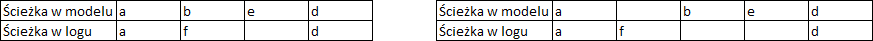
\includegraphics[scale=0.7]{bad-alignment.png}}
	\caption{\label{fig:bad-alignment}Nieprawidłowe odwzorowanie}
\end{figure}
Dla pozostałych wariantów odwzorowanie jest pełne i błąd wynosi 0:
\begin{figure}[h]
	\centering{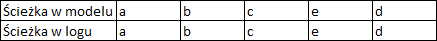
\includegraphics[scale=0.7]{good-alignment.png}}
	\caption{\label{fig:good-alignment}Prawidłowe odwzorowanie}
\end{figure}
\newline Podstawiając wszystkie odwzorowania do wzoru:
\begin{center}
\begin{tabular}{l}
$blad\_odwzorowania = \frac{2 * \frac{0}{5 +\ 5} + \frac{0}{4 +\ 4} + \frac{0}{5 +\ 5} + \frac{3}{4 +\ 3}}{22} = 0.0195$ \\

$M_o = (1 - 0.0195)^4 = 0.9243$
\end{tabular}
\end{center}

\subsubsection{Obliczanie precyzji}
Potrzebna jest ilość osiągalnych kolejnych zdarzeń dla danej aktywności. Zależy ona od kontekstu, w jakim dana aktywność jest wykonywana np. dla bramki I - AND można jako kolejne wykonać tyle aktywności, ile nie zostało do tej pory wykonanych w tej bramce, z wyjątkiem ostatniej i gdzie przechodzimy do kolejnych aktywności spoza bramki. Dla demonstrowanego przykładu wygląda to następująco:

\begin{figure}[h]
	\centering{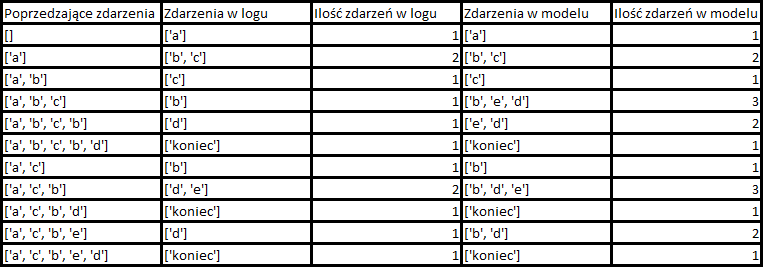
\includegraphics[scale=0.7]{precision-calculation.png}}
	\caption{\label{fig:directly-follows}Kolejne zdarzenia}
\end{figure}

Podstawiając te dane do wzoru:
\begin{center}
$M_{pre} = (1 - (\frac{1\ -\ 1}{1}\ +\ \frac{2\ -\ 2}{2}\ +\ \frac{1\ -\ 1}{1}\ +\ \frac{3\ -\ 1}{3}\ +\ \frac{2\ -\ 1}{2}\ +\ \frac{1\ -\ 1}{1}\ +\ \frac{1\ -\ 1}{1}\ +\ \frac{3\ -\ 2}{3}\ +\ \frac{1\ -\ 1}{1}\ +\ \frac{2\ -\ 1}{2}\ +\ \frac{1\ -\ 1}{1}))^{\frac{1}{3}} = 0.9465 $
\end{center}

\subsubsection{Obliczanie generalizacji}
Słabością tej metryki jest to, że wpływa na nią rozmiar dziennika zdarzeń. Jeśli ilość rekordów jest mała, jak w powyższym przykładzie, to generalizacja będzie słaba. Starając się znaleźć najlepszy model dla danego dziennika zdarzeń, on pozostaje stały, więc nie wpływa to na prawidłowość rozwiązania. W tym przypadku:
\begin{center}
$M_g = 1 - \frac{(\frac{1}{\sqrt{5}}\ +\ \frac{1}{\sqrt{4}}\ +\ \frac{1}{\sqrt{4}}\ +\ \frac{1}{\sqrt{2}}\ +\ \frac{1}{\sqrt{1}}\ +\ \frac{1}{\sqrt{5}})}{6} = 0.3997$
\end{center}

\subsubsection{Obliczanie złożoności}
Najpierw obliczana jest złożoność dla poszczególnych bramek, co jest konieczne na wcześniejszym etapie działania algorytmu, a następnie te wartości są podstawiane do wzoru wraz z błędem dopasowania obliczonym w sekcji \ref{sec:alignment-calculation}:\newline
$zlozonosc\_dla\_bramki\_AND = 2! = 2$\newline
$zlozonosc\_dla\_bramki\_OR = 2! * \frac{2!}{(2! * (2 - 2)!)} + 1! *  \frac{2!}{(1! * (2 - 1)!)} + 0! * \frac{2!}{(0! * (2 - 0)!)} = 2 + 2 + 1 = 5$\newline
$zlozonosc = 1 * 2 * 5 * 1 = 10$
\begin{center}
$M_z = 1 - \frac{1}{\sqrt{1 + 0.0195\ *\ \sqrt{10}}} = 0.9706$
\end{center}